\section{Group Theory (6G6Z3012)}\label{group-theory-6g6z3012}

\subsection{What is a group?}\label{what-is-a-group}

A set $G$ with a binary operation $\star$ satisfying

\begin{itemize}
\itemsep1pt\parskip0pt\parsep0pt
\item
  $G$ is a closed system under $\star$,
\item
  $\star$ is associative on $G$,
\item
  $G$ contains an identity element for $\star$,
\item
  $G$ contains inverse elements for $\star$ .
\end{itemize}

Groups arise in many different contexts in mathematics.

\subsection{Syllabus topics}\label{syllabus-topics}

\subsubsection{Introduction to group
theory:}\label{introduction-to-group-theory}

Binary operations on sets and definition of a group with examples.
Cayley tables.

\subsubsection{Examples of groups:}\label{examples-of-groups}

Symmetry groups of two and three-dimensional objects, the dihedral
groups $D_n$, rotational symmetry groups of three-dimensional polyhedra.
Permutation groups, the Symmetric groups $S_n$ and the Alternating
groups $A_n$. Number based groups under arithmetic operations, the
cyclic groups $\mathbb{Z}_n$. Groups of matrices.

\subsection{Rotational symmtry groups of 2D \& 3D solids (4D, 5D,
\ldots{} ?)}\label{rotational-symmtry-groups-of-2d-3d-solids-4d-5d}

\subsubsection{Visualising the elements of
$\Gamma^+(T)$}\label{visualising-the-elements-of-gammat}

\begin{figure}[htbp]
\centering
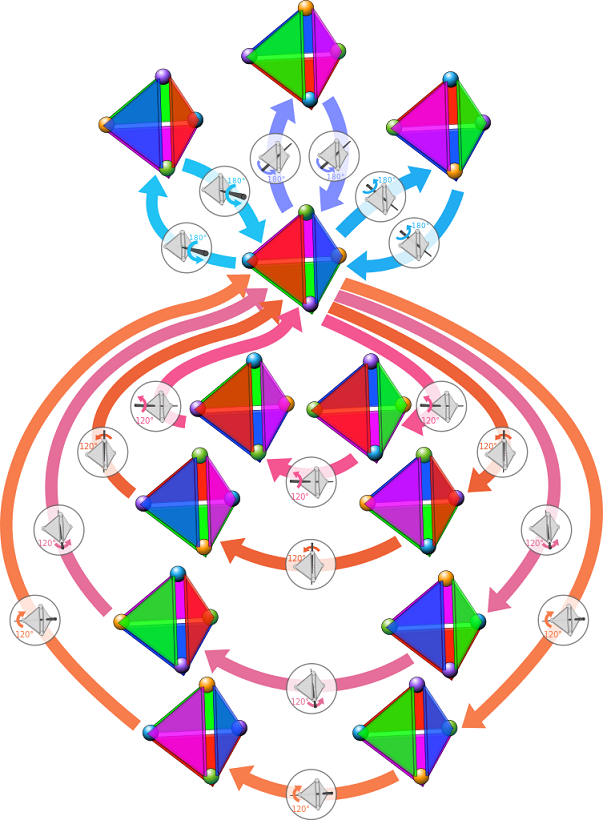
\includegraphics{./tetrahedrons.png}
\caption{Symmetries of a tetrahedron}
\end{figure}

\subsection{The Symmetric group, $S_4$, on four
objects}\label{the-symmetric-group-sux5f4-on-four-objects}

\begin{figure}[htbp]
\centering
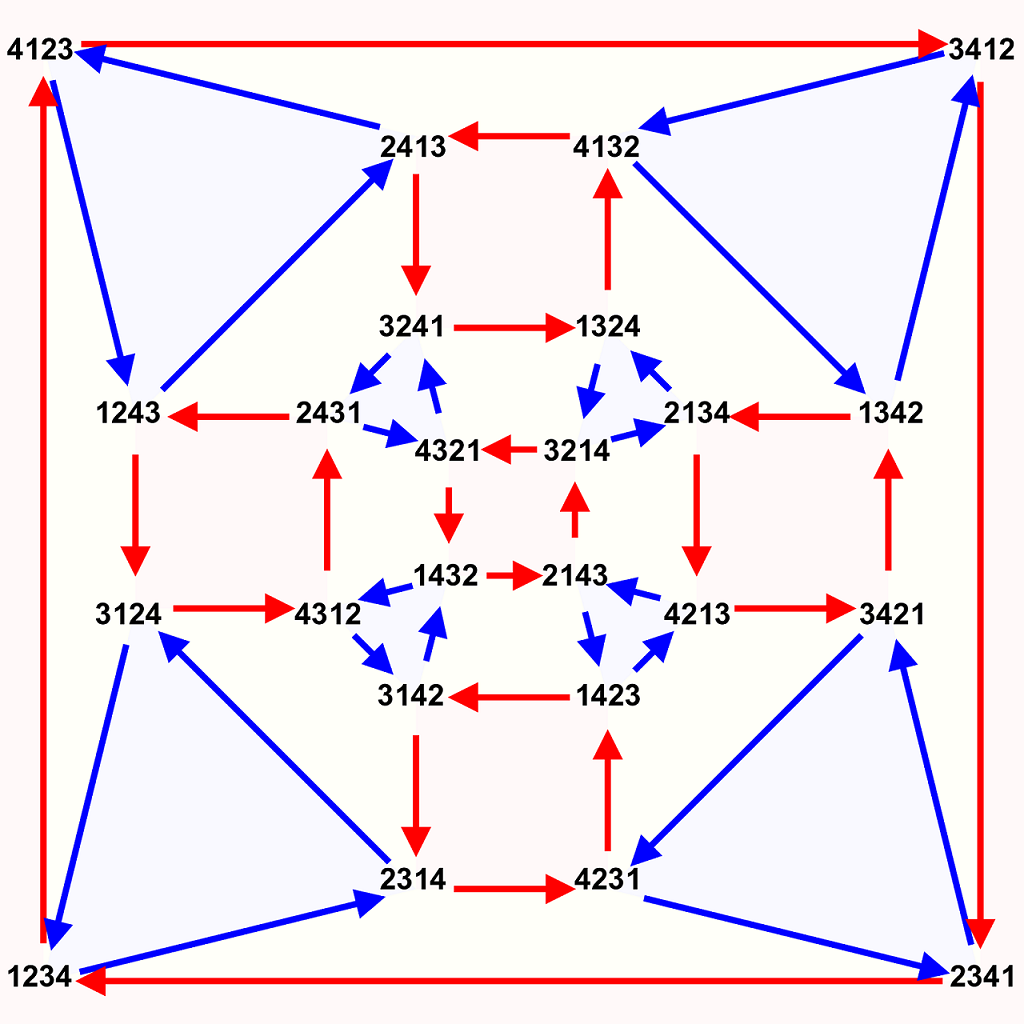
\includegraphics{./S4_Cayley.png}
\caption{Cayley graph of S\_4}
\end{figure}

\subsection{Syllabus topics}\label{syllabus-topics-1}

\subsubsection{Initial group theory:}\label{initial-group-theory}

Various concept definitions and examples, including: elements, orders,
Abelian groups, subgroups, generators and cyclic/non-cyclic. The natural
mappings between groups, homomorphisms and isomorphisms. Examples of
isomorphic pairs and non-isomorphic pairs. Cayley's theorem: Every group
isomorphic to a group of permutations.

\subsubsection{Classification problems:}\label{classification-problems}

What are the grand enterprises of group theory? What classification
problems can be posed?

\subsubsection{Lagrange's theorem:}\label{lagranges-theorem}

Restricting the possibilities for subgroup orders. Equivalence
relations, equivalence classes, cosets. Normal groups and quotient
groups.

\subsection{Lagrange's theorem}\label{lagranges-theorem-1}

\begin{figure}[htbp]
\centering
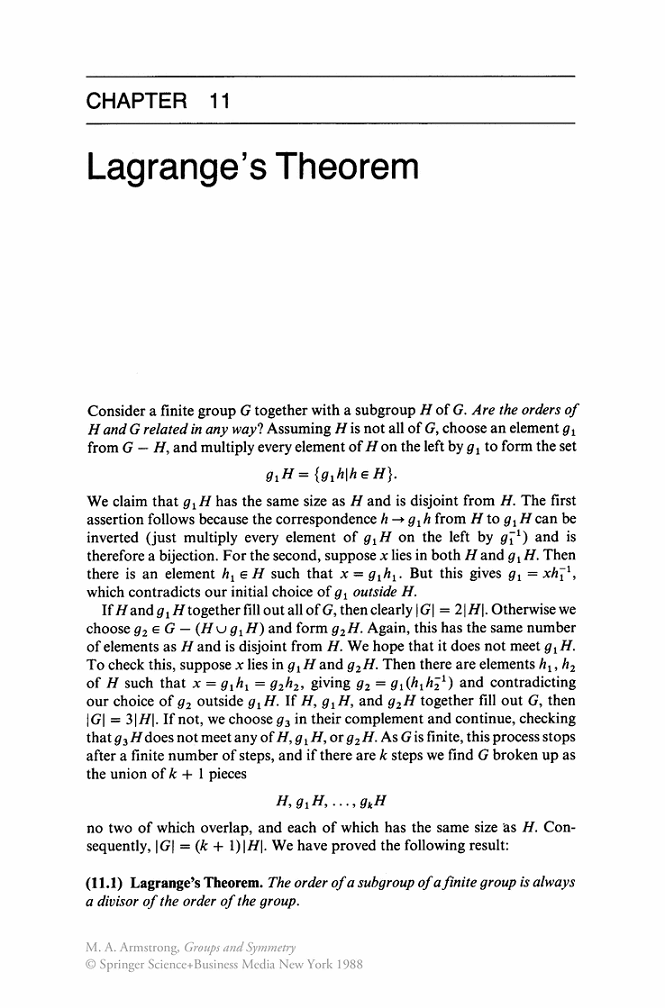
\includegraphics{./MAA.png}
\caption{MAArmstrong}
\end{figure}

\subsection{Syllabus topics}\label{syllabus-topics-2}

\subsubsection{Group presentations:}\label{group-presentations}

How to systematically describe groups in a computable way. Group
presentations, generators and relations, presentation matrices. The
isomorphism decision problem based on matrices.

\subsubsection{The classification of finitely presented Abelian
groups:}\label{the-classification-of-finitely-presented-abelian-groups}

A matrix reduction algorithm to decide the isomorphism problem amongst
finitely presented Abelian groups. The canonical form of finitely
presented Abelian group as a direct sum of cyclic groups.

\subsubsection{Classification of groups of low
order:}\label{classification-of-groups-of-low-order}

What about non-Abelian groups? Why we can't solve using matrix
reduction? Investigation of groups of low order and enumeration and
classification of all groups up to some suitable order.

\subsubsection{Sylow's theorems:}\label{sylows-theorems}

Discussion of the converse to Lagrange's theorem. Group actions, orbits,
stabilizers. Self-action by conjugation. Sylow's theorems.

\subsection{Wider interst material /
applications}\label{wider-interst-material-applications}

The unit could contain interesting general material on the following
topics/applications.

\subsubsection{The classification of finite simple
groups}\label{the-classification-of-finite-simple-groups}

The grand project. Status of the proof. Some history and biographical
details of the completion of the project. The families in the
classification. The sporadic groups. The Monster group and Monstrous
Moonshine.

\paragraph{The Monster group}\label{the-monster-group}

A group, $M$, with approx. $8 \times 10^{53}$ elements, that is
\emph{simple}, i.e.~it has no \emph{normal} subgroups.

$M$ is (isomorphic to) a group of rotations of 196883-dimensional space.

$M$ is (isomorphic to) a group of matrices generated by two particular
binary $196882 \times 196882$ matrices.

\subsubsection{Algorithmic problems}\label{algorithmic-problems}

The word problem. Computability. Alan Turing.

\begin{figure}[htbp]
\centering
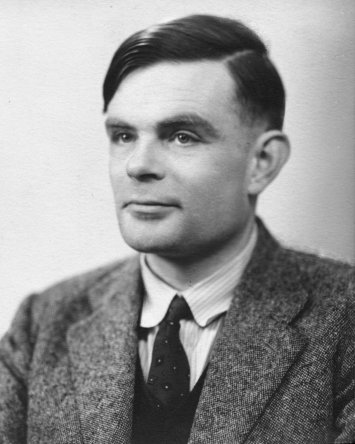
\includegraphics{turing.jpg}
\caption{Alan Turing}
\end{figure}

\subsubsection{Combinatorial enumeration and geometric classification
problems}\label{combinatorial-enumeration-and-geometric-classification-problems}

Counting number of distinguishable colourings of geometric objects.
Classifying the symmetry types of two-dimensional wallpaper patterns.
Classifying two and three-dimensional crystal structures (lattices).

\subsubsection{Galois theory}\label{galois-theory}

\begin{figure}[htbp]
\centering
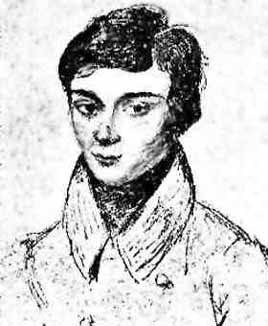
\includegraphics{./Galois.jpeg}
\caption{Galois}
\end{figure}

Life of Galois (1811 - 1832). Galois theory. Formulas for roots of
polynomials. Construction problems with ruler and compass.

\subsection{Teaching team, teaching pattern \&
assessment}\label{teaching-team-teaching-pattern-assessment}

\begin{itemize}
\item
  Unit designed by Killian O'Brien \& Seamus O'Shea
\item
  Taught by Killian , \ldots{}
\item
  2 hours lecture + 1 hour tutorial (or sometimes computer lab) per
  week.
\item
  Assessment is by Coursework Report (40\%) and Summer Exam (60\%).
\end{itemize}

\subsection{Nature of the unit}\label{nature-of-the-unit}

\begin{itemize}
\item
  A thorough introduction to a substantial area of pure mathematics that
  has strong connections to areas of geometry, combinatorics, graph
  theory, \ldots{} .
\item
  Definately suited to students who like problem solving and the unit
  will develop your skills in this area.
\item
  We will use the Sage mathematics system to aid our investigations. You
  will also get an introduction to the Python programming language.
  (\href{http://www.sagemath.org}{www.sagemath.org},
  \href{https://cloud.sagemath.org}{cloud.sagemath.org},
  \href{https://sagecell.sagemath.org}{sagecell.sagemath.org})
\end{itemize}
